\chapter{Resultados preliminares na GPU}\label{apdx:oneMaxNaGPU}
	
	\textbf{Resumo}\footnote{Esses resultados foram apresentados na III Escola Regional de Alto Desempenho São Paulo (ERAD-SP 2012).}: Apresento uma implementação paralela dos operadores do algoritmo genético utilizando a arquitetura CUDA, em que cada indivíduo foi associado a uma única \emph{thread}. Ao aplicá-la ao problema ONEMAX, observei ganhos de desempenho promissores (>10x). Os pontos fracos e possíveis estratégias de melhoria são discutidos.
	
	---
	
		O GA aqui desenvolvido buscou a solução do problema ONEMAX, cujo objetivo é encontrar uma sequência de $N$ bits com a maior quantidade possível de “1” a partir de uma sequência aleatória de “1” e “0”. O ONEMAX é especialmente indicado para o início dos estudos em GA. Além de permitir simples implementação, possui representação cromossomial binária que, junto com o crossover de ponto único, forma a base da teoria original de Holland \cite{Linden2008}.

	O programa paralelizado foi uma tradução literal do seu equivalente serial para a sintaxe do CUDA C. Ou seja, não houve nenhuma mudança estrutural no código, seja nas variáveis e estruturas de dados, seja na ordem de execução das funções e procedimentos. Apenas o preenchimento aleatório da população inicial é executado na CPU, de forma que o núcleo do programa é executado inteiramente na GPU \cite{onemaxNaGPU}. 

	A população do GA era constituída por indivíduos formados por cromossomos com \textit{\texttt{numGenes}} elementos do tipo \texttt{char}. Cada elemento do vetor (gene) podia ter um valor  “1” ou “0”. Dentro do problema ONEMAX, os melhores indivíduos foram os que apresentaram maior número de genes iguais a “1”.
		
	\begin{figure}[htbp]
		\centering
			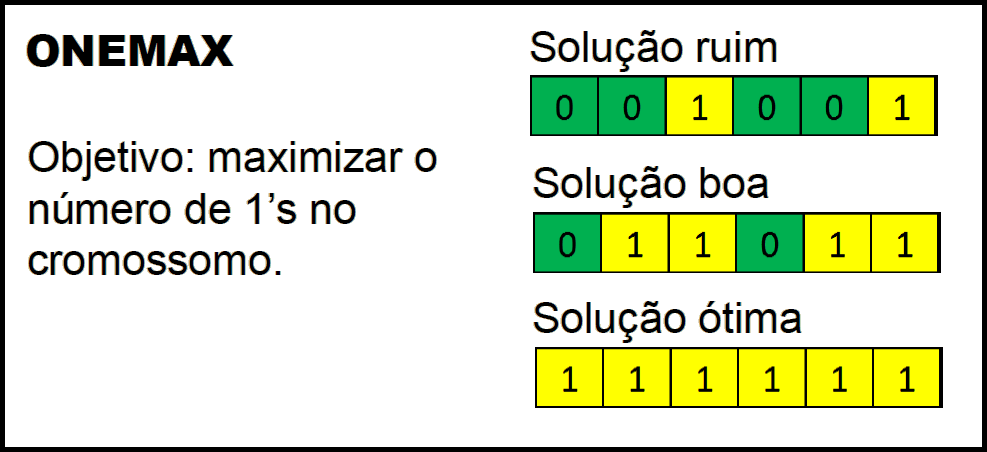
\includegraphics[width=0.50\textwidth]{figs/resultados/onemax/onemax_objetivo.png}
		\caption{ONEMAX, um problema clássico nos Algoritmos Genéticos.}
		\label{fig:onemax_objetivo}
	\end{figure}
		
	Implementei um \emph{kernel} (função que tem sua execução feita pela GPU) para cada um dos quatro passos do GA: cálculo da função avaliadora (\emph{fitness}), seleção, \emph{crossover} e mutação. Eles são chamados um após o outro até que um número máximo de gerações seja atingido. Isso é feito dentro do \emph{loop} principal (realizado na CPU), mas sem troca de informação entre CPU e GPU.
	
	No início do programa duas gerações são alocadas na memória global da GPU, as quais são usadas alternadamente como \emph{input} e \emph{output} dos kernels. Apenas as chamadas dos kernels acontecem na CPU, enquanto o restante (execução + dados) está na GPU. Todos os \emph{kernels} tinham como \emph{input} e \emph{output} uma estrutura do tipo Geração. Ou seja, as funções operaram sobre toda a população do GA, levando-nos a adotar como estratégia o paralelismo no nível dos indivíduos.
	
	\begin{figure}[htbp]
		\centering
			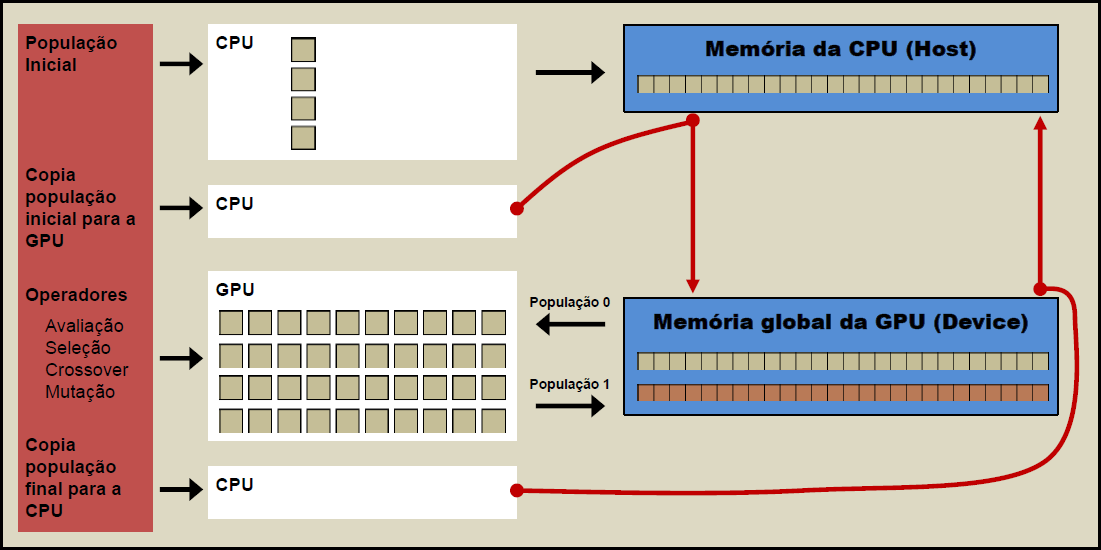
\includegraphics[width=1.00\textwidth]{figs/resultados/onemax/onemax_execucao.png}
		\caption{Execução do ONEMAX paralelo. Apenas as chamadas dos kernels acontecem na CPU, enquanto o restante (execução + dados) está na GPU.}
		\label{fig:onemax_execucao}
	\end{figure}
		
	No cálculo do \emph{fitness}, o \emph{input} foi uma população com \textit{\texttt{numIndividuos}} e o \emph{output} uma população com os mesmos \textit{\texttt{numIndividuos}} e suas respectivas notas. O cálculo do \emph{fitness} de cada indivíduo foi realizado por meio da soma dos valores de seus genes. Por exemplo, para um indivíduo formado por um cromossomo de 6 genes \mbox{(\textit{\texttt{numGenes}} = 6)} com a configuração “010101”, o valor do fitness é 3 e a solução ótima para este caso seria “111111” (figura \ref{fig:onemax_objetivo}). No código serial a programação é simples e envolve apenas um laço \texttt{\textbf{\textit{for}}} que percorre o cromossomo e soma os bytes. Porém, note que toda informação necessária para esse cálculo está contida no próprio cromossomo, ou seja, a obtenção do \emph{fitness} de um dado indivíduo não depende do restante da população. Assim, a paralelização do cálculo do \emph{fitness} deu-se por meio da associação de uma \emph{thread} para cada indivíduo.
	
	Para o operador de seleção, optei pela seleção via torneio com o tamanho do torneio fixo e igual a dois. Novamente, o \emph{input} e o \emph{output} são populações. Na entrada há \textit{\texttt{numIndividuos}} e suas notas. Os mais aptos (maiores \emph{fitness}) têm maiores chances de serem selecionados, e compõem os \textit{\texttt{numIndividuos}} da população na saída. Assim como no cálculo do \emph{fitness}, o paralelismo acontece no nível dos indivíduos. Para cada indivíduo na população de saída há uma \emph{thread}, que seleciona aleatoriamente dois cromossomos na população da entrada (memória global) e fica com o de maior \emph{fitness}.

O \emph{input} do \emph{crossover} é a população resultante da seleção. Utilizei o \emph{crossover} de dois pontos, independentemente da quantidade de genes do cromossomo, com probabilidade $p_C = 90\%$. Na implementação serial, apenas um indivíduo é gerado ao término do \emph{crossover}. Isso garantiu que, na versão paralela, a chamada da função de \emph{crossover} fosse configurada com exatamente o mesmo número de \emph{threads} dos operadores anteriores (avaliação e seleção): uma \emph{thread} para cada indivíduo na população de saída, que recebe um cromossomo resultante do \emph{crossover}.

Após o \emph{crossover} todos os indivíduos passam por uma mutação simples, onde cada gene do cromossomo tem baixa probabilidade (0,01\%) de ser invertido (0 $\rightarrow$ 1 ou 1 $\rightarrow$ 0). Logo, semelhante ao cálculo do \emph{fitness}, a mutação em um dado indivíduo é independente do restante da população. Mais uma vez, uma \emph{thread} foi associada a cada \textit{\texttt{iIndividuo}} cromossomo na saída, que recebe os genes modificados do \textit{\texttt{iIndividuo}} na entrada. 

	Os experimentos foram executados em um laptop equipado com uma CPU Intel Core 2 Duo T6600 - 2,2 GHz. A placa de vídeo utilizada foi uma GeForce G 130M, com quatro multiprocessadores a 1,5 GHz e memória global total de 466 MB. A versão da API CUDA foi a 4.0, programada com o Microsoft Visual C++ Express 2008.
	
	A placa G 130M possui capacidade de computação 1.1 (que indica a versão do hardware de computação presente na GPU). Comparada com a primeira versão (arquitetura original da G80), ela adiciona suporte à operações na memória global que permitem que múltiplas \emph{threads} executem, sem conflito, operações ler-modificar-escrever na memória. Como o suporte às operações de ponto flutuante com precisão dupla só foi disponibilizado na versão 1.3, tanto o programa serial quanto o paralelo utilizaram precisão simples.
	
	As medidas de desempenho foram feitas com o objetivo de observar a influência de dois parâmetros do GA: i) número de indivíduos na população e ii) tamanho do cromossomo. O ganho na velocidade foi calculado como a razão entre o tempo de execução do programa serial e o tempo de execução do programa paralelo.

Verifiquei que o ganho de desempenho da versão paralela do GA cresce com o aumento do número de indivíduos (figura \ref{fig:ganhoNumInd}). O programa serial é mais rápido (ganho < 1) para populações pequenas (< 50). Porém, a partir de uma população de 50 indivíduos, o programa paralelo apresenta desempenho superior. Com 600 indivíduos, a versão paralela é oito vezes mais rápida para um cromossomo de tamanho 10, e dez vezes para um cromossomo de tamanho 300. 

\begin{figure}[htbp]
	\centering
		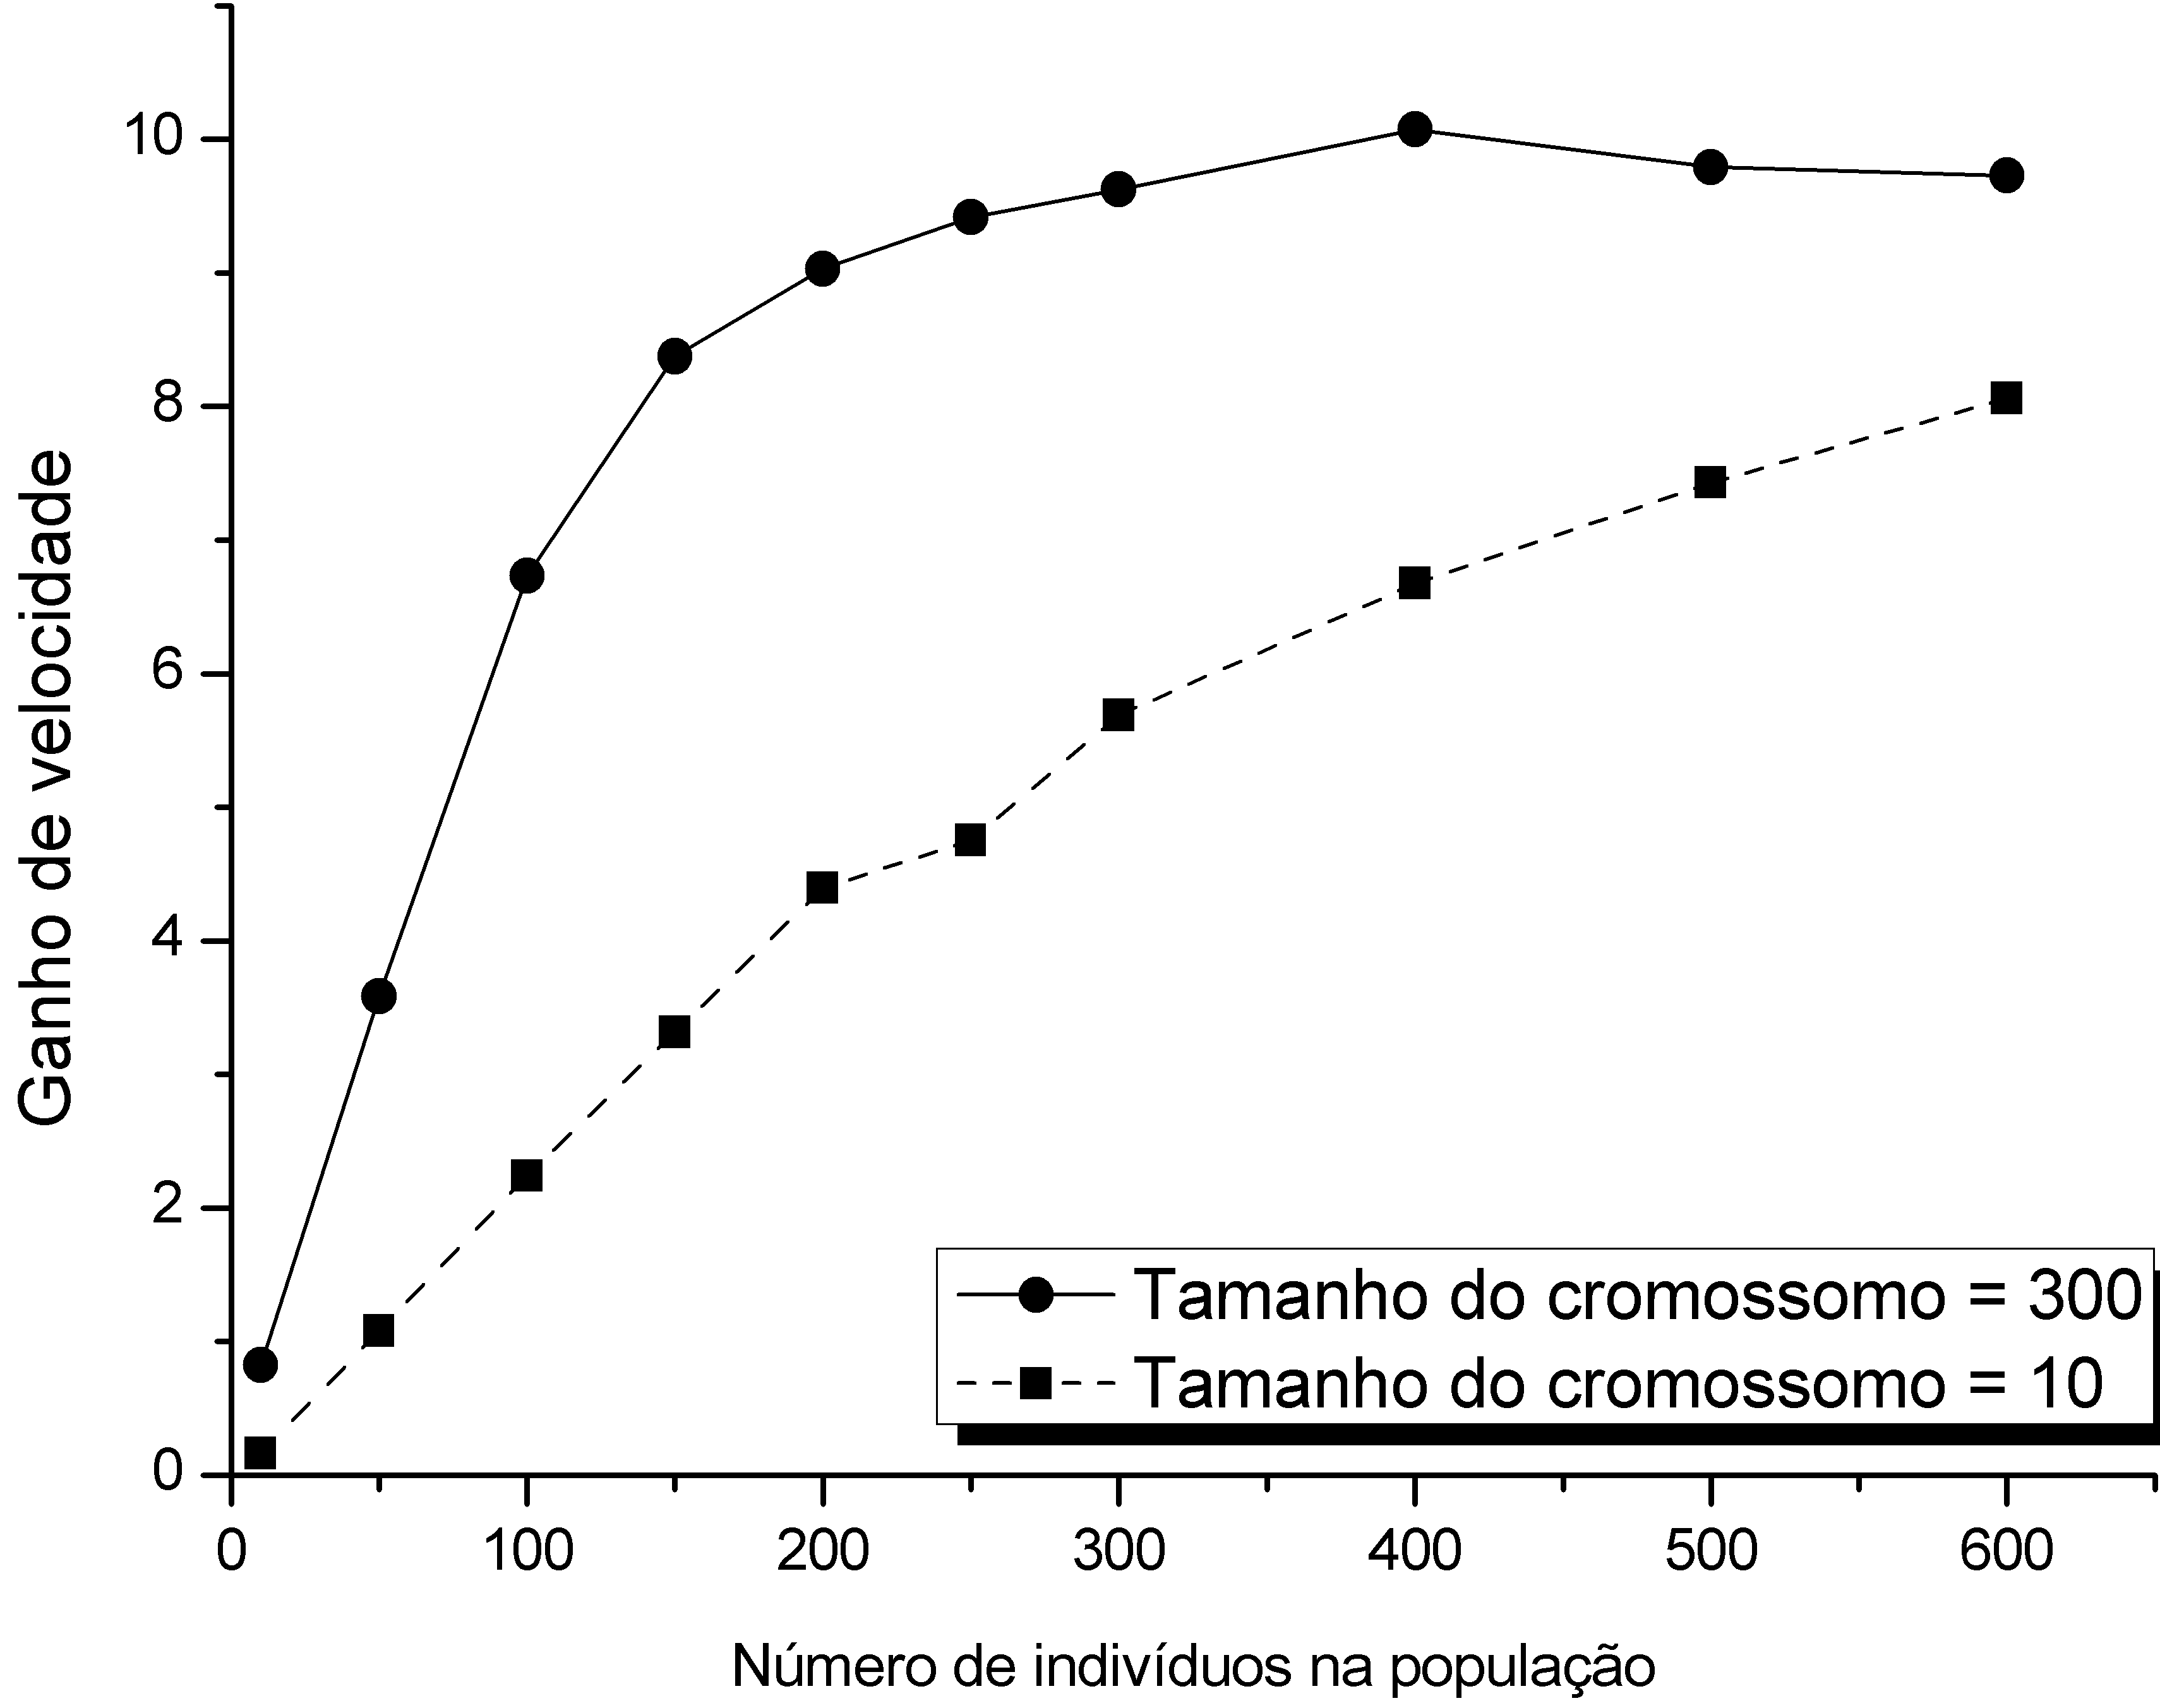
\includegraphics[width=0.70\textwidth]{figs/resultados/onemax/ganhoNumInd.png}
	\caption{ONEMAX paralelo. Ganho de velocidade em função do número de indivíduos da população.}
	\label{fig:ganhoNumInd}
\end{figure}

	Ao analisar a influência do tamanho do cromossomo, verifiquei um comportamento aproximadamente constante do ganho (figura \ref{fig:ganhoTamCromo}). Isso era esperado, pois a paralelização ocorreu no nível dos indivíduos e não no nível dos cromossomos. Com 600 indivíduos o ganho fica em torno de nove vezes para qualquer tamanho de cromossomo. O comportamento repete-se com uma população de 10 indivíduos, mas, nesse caso, o programa serial sempre é mais rápido, mesmo para cromossomos muito pequenos (ganho sempre \mbox{< 1}). 
		
	\begin{figure}[htbp]
		\centering
			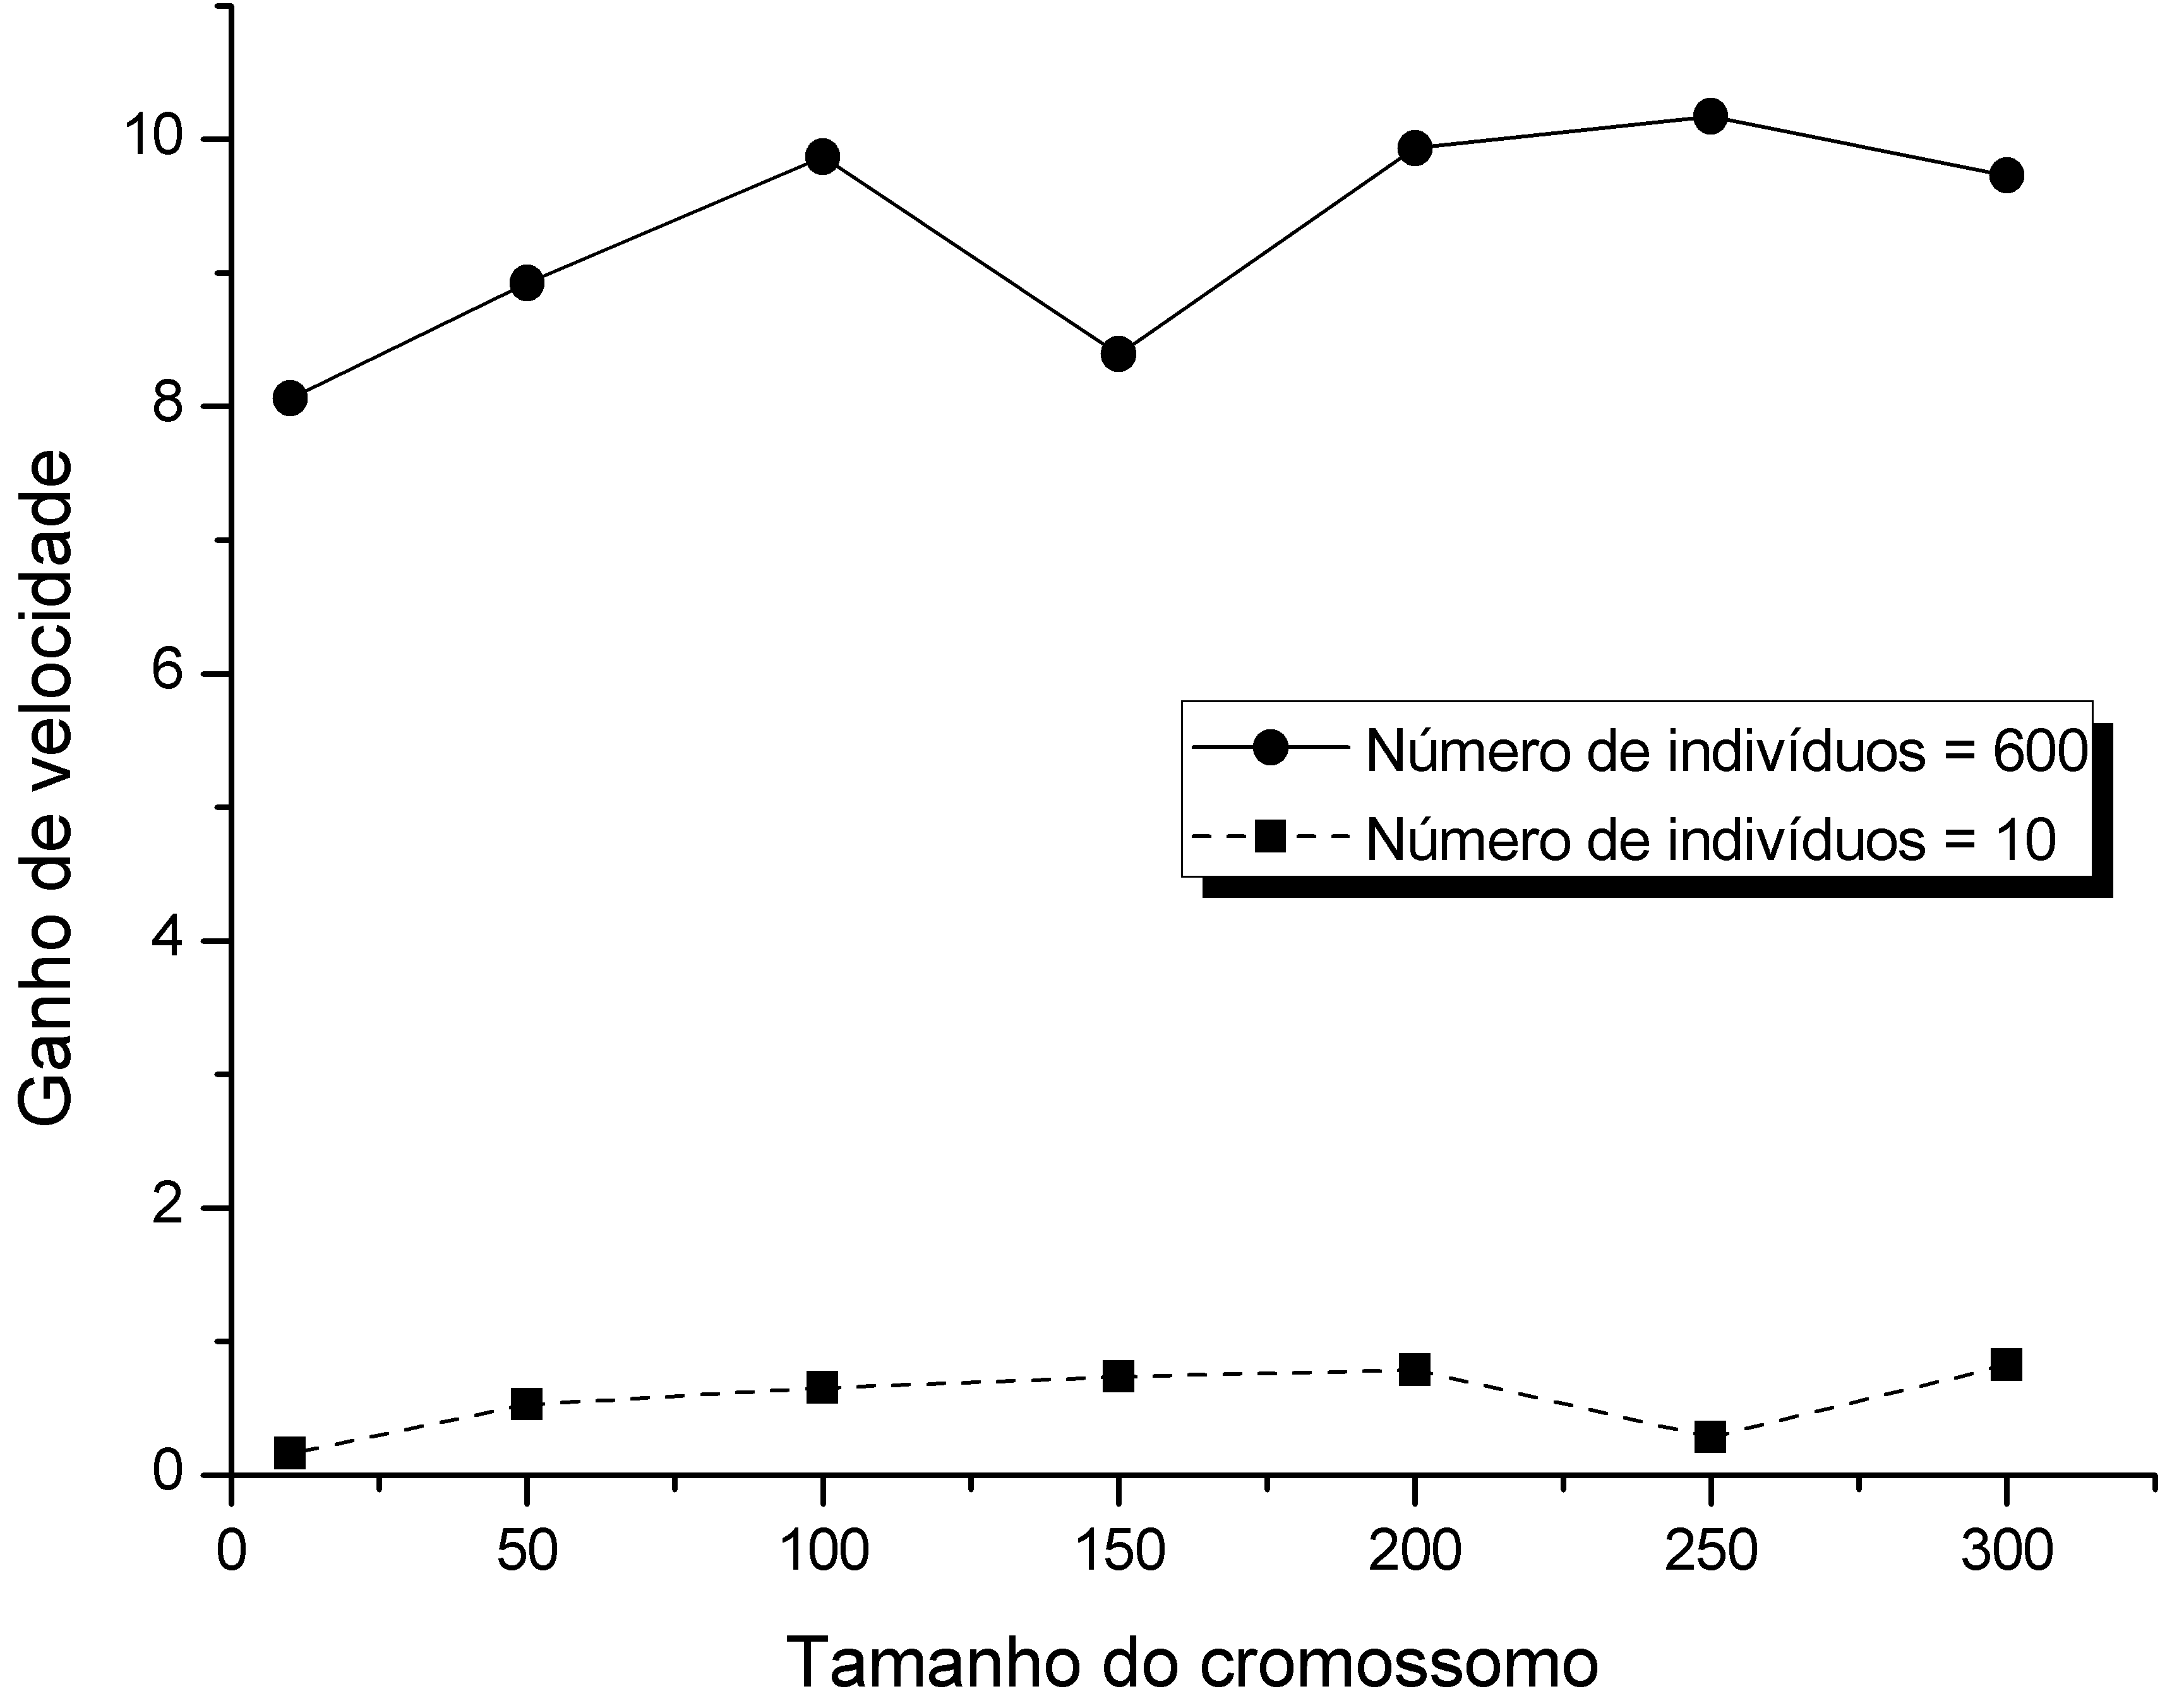
\includegraphics[width=0.70\textwidth]{figs/resultados/onemax/ganhoTamCromo.png}
		\caption{ONEMAX paralelo. Ganho de velocidade em função do tamanho do cromossomo.}
		\label{fig:ganhoTamCromo}
	\end{figure}